\documentclass[11pt,a4paper]{article}
\usepackage[T1]{fontenc}
\usepackage[utf8]{inputenc}
\usepackage[spanish,es-tabla]{babel}
\usepackage{lmodern,microtype}
\usepackage[margin=2.2cm]{geometry}
\usepackage{graphicx,xcolor,booktabs,tabularx,longtable,array,float,caption}
\usepackage{csquotes}
\usepackage[backend=biber,style=ieee,sorting=none,maxbibnames=99,doi=true,url=true]{biblatex}
\addbibresource{referencias.bib}
\DefineBibliographyStrings{spanish}{artno={art.}}
\DeclareBibliographyDriver{online}{%
  \usebibmacro{bibindex}\usebibmacro{begentry}%
  \usebibmacro{author/editor+others/translator+others}%
  \setunit{\adddot\addspace}\usebibmacro{title}%
  \setunit{\adddot\addspace}\printfield{version}%
  \newunit\newblock\printlist{organization}%
  \setunit{\addcomma\addspace}\usebibmacro{date}%
  \setunit{\adddot\addspace}\usebibmacro{url+urldate}%
  \usebibmacro{finentry}}
\usepackage[hidelinks,unicode]{hyperref}
\hypersetup{pdftitle={Análisis crítico de NATS con JetStream frente a Apache Pulsar},pdfauthor={Nixon Antonio Piguave Montaño}}
\definecolor{azul}{HTML}{17344B}
\usepackage{titlesec}
\titleformat{\section}{\large\bfseries\color{azul}}{\thesection.}{0.6em}{}
\titleformat{\subsection}{\normalsize\bfseries\color{azul}}{\thesubsection.}{0.6em}{}
\setlength{\parindent}{0pt}
\setlength{\parskip}{5pt}
\renewcommand{\arraystretch}{1.15}
\captionsetup{font=small,labelfont=bf}
\setlength{\emergencystretch}{2em}
\newcolumntype{Y}{>{\raggedright\arraybackslash}X}
\newcommand{\archivo}[1]{\texttt{\detokenize{#1}}}
\newcommand{\captura}[4]{\begin{figure}[H]\centering\includegraphics[width=\linewidth,height=#4\textheight,keepaspectratio]{#1}\caption{#2}\label{#3}\end{figure}}

\begin{document}
\begin{titlepage}
\centering
{\Large\bfseries Universidad Técnica Estatal de Quevedo\par}
\vspace{0.35cm}
{\large Facultad de Ciencias de la Computación\par}
{\large Carrera de Software\par}
\vspace{2cm}
{\Large\bfseries TA-IND-01\par}
\vspace{0.5cm}
{\LARGE\bfseries Análisis crítico de NATS con JetStream frente a Apache Pulsar\par}
\vspace{0.7cm}
{\large Replicación, comunicación y recuperación ante la caída de un nodo\par}
\vspace{1.7cm}
\begin{tabular}{rl}
\textbf{Asignatura:} & Aplicaciones Distribuidas\\[6pt]
\textbf{Estudiante:} & Nixon Antonio Piguave Montaño\\[6pt]
\textbf{Curso y paralelo:} & 7mo nivel, paralelo A\\[6pt]
\textbf{Fecha:} & 14 de noviembre de 2026
\end{tabular}
\vfill
\textbf{Repositorio público}\par
\small\url{https://github.com/NixonPiguave/app-dist-TA-IND-01-}\par
\vspace{0.2cm}
Carpeta de la entrega: \archivo{nixon/}
\end{titlepage}
\pagenumbering{arabic}

\section*{Resumen}
Este informe analiza NATS con JetStream y lo compara con Apache Pulsar mediante los conceptos de distribución de la Unidad 1. Se combinan artículos científicos, documentación técnica y una prueba local ejecutada con Docker en Windows. El experimento utiliza tres servidores, un flujo con tres copias y dos mensajes identificables. Primero se comprueba la comunicación del clúster; después se termina abruptamente el proceso que dirige el flujo, se realizan operaciones con los nodos supervivientes y se reincorpora el nodo detenido. Las salidas muestran un nuevo líder, recuperación del mensaje anterior, aceptación de otro mensaje y sincronización posterior de las réplicas. Estos resultados respaldan la tolerancia al fallo de un proceso en las condiciones probadas, sin demostrar disponibilidad continua ni resistencia a la pérdida de toda la computadora. La comparación distingue el consenso del flujo en JetStream de la separación entre servicio y almacenamiento en Pulsar. Se concluye que la elección depende del alcance del fallo, las confirmaciones requeridas y la operación del sistema, y que disponer de varias copias no elimina la necesidad de definir sus garantías.

\section{Introducción}
Una aplicación que recibe solicitudes y procesa cada una hasta el final puede obligar al usuario a esperar por tareas que no necesitan terminar en la misma respuesta. La mensajería permite separar la recepción de un evento de su tratamiento posterior. NATS con JetStream aborda este problema añadiendo almacenamiento y recuperación de mensajes a la infraestructura de comunicación de NATS. La pregunta de este trabajo es qué parte de esa separación sigue funcionando cuando desaparece el proceso que dirige un flujo y qué condiciones limitan esa continuidad.

Existen aplicaciones documentadas cercanas a este problema. Ma’soem y Rukhviyanti estudian un prototipo de recolección de respuestas de exámenes con 300 usuarios sintéticos: JetStream actúa como intermediario persistente y la API responde antes de completar el procesamiento posterior \cite[pp.~485, 493]{masoem2026}. Es una escala experimental de la aplicación, no una medición de la capacidad máxima de NATS. Ju, Seo y Kim emplean JetStream en una plataforma IoT con un clúster de gestión y tres clústeres miembros \cite[pp.~7--8]{Ju2026}. Sus usuarios objetivo son aplicaciones que reciben eventos de sensores y disparan funciones distribuidas; los resultados pertenecen a esa plataforma completa.

Elegí NATS porque podía ejecutarlo localmente, observar sus réplicas y provocar una caída controlada. Apache Pulsar resuelve un problema comparable de publicación, conservación y entrega de mensajes, pero separa los brokers de su almacenamiento BookKeeper. El análisis de Pulsar es documental; no se ejecutó un segundo laboratorio. La comparación combina mecanismos y resultados publicados, sin presentar las condiciones de esos estudios como si fueran iguales a las de mi computadora.

\section{Arquitectura y comunicación}
\subsection{Del bosquejo al despliegue local}
El bosquejo del Anexo~\ref{anexo:a} representa un cliente y tres nodos con copias del mismo flujo. La figura~\ref{fig:arquitectura} conserva esa estructura y añade nombres reales, almacenamiento, puertos y el límite físico del experimento. La configuración reproducible es \archivo{experimento/compose-cluster.yaml}. Cada contenedor ejecuta \archivo{nats:2.15.3-alpine}, habilita JetStream y dispone de un volumen propio montado en \archivo{/data}. El cliente temporal utiliza \archivo{natsio/nats-box:0.19.7}.

\begin{figure}[H]
\centering
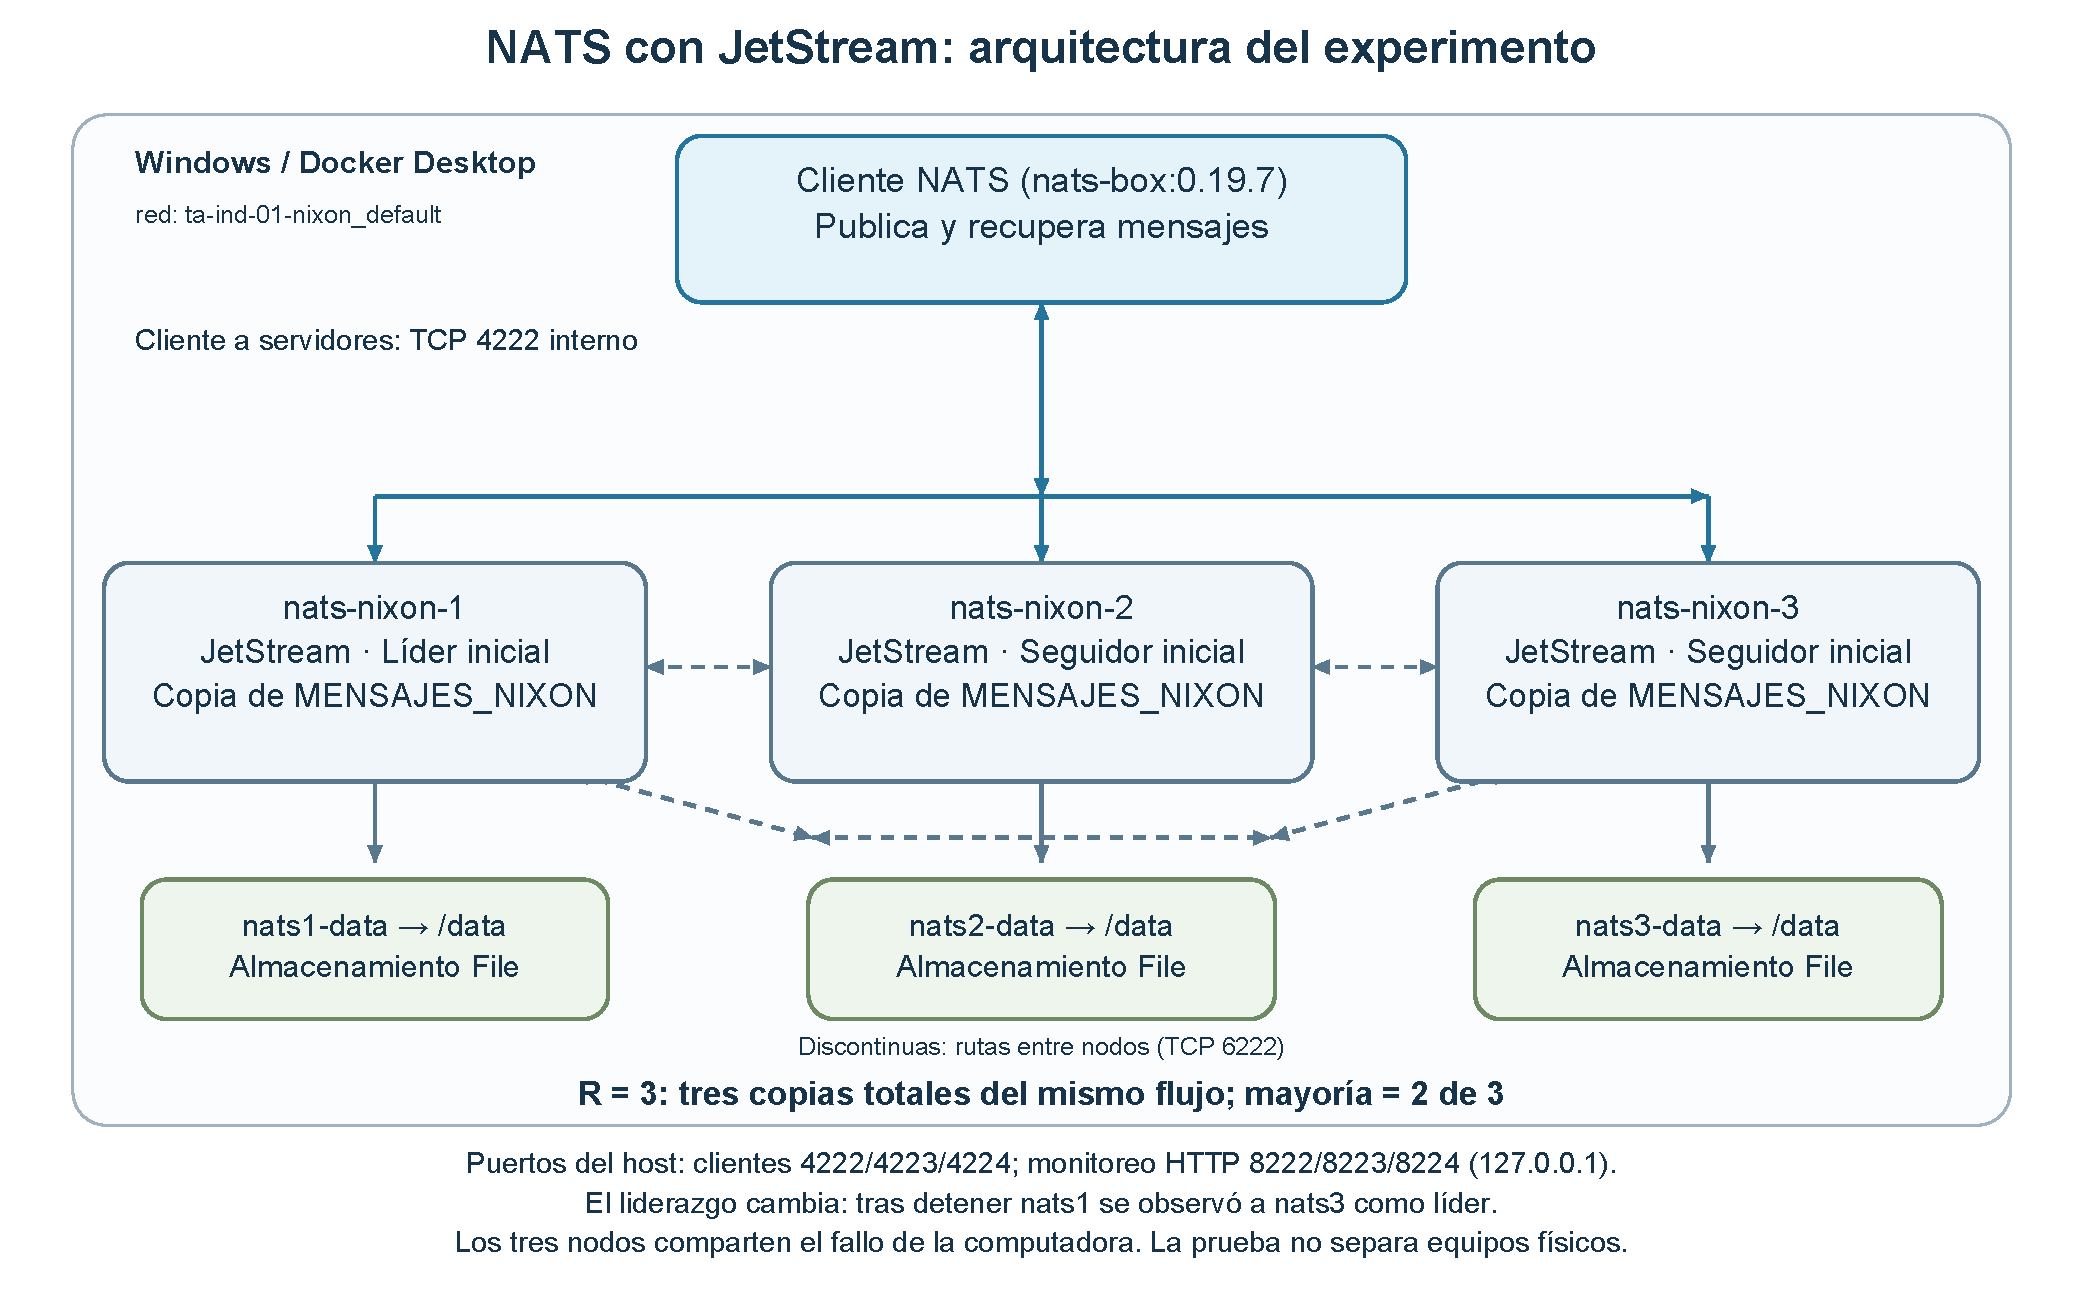
\includegraphics[width=\linewidth]{figuras/arquitectura.pdf}
\caption{Arquitectura digital derivada del bosquejo y de la configuración ejecutada. Tres copias totales del flujo; los roles corresponden al estado inicial observado. Fuente conceptual: documentación de JetStream \cite{natsCluster,natsReplicacion}.}
\label{fig:arquitectura}
\end{figure}

Los servicios \archivo{nats1}, \archivo{nats2} y \archivo{nats3} se comunican por rutas internas en el puerto TCP 6222. Todos mantienen una copia de \archivo{MENSAJES_NIXON}, asociado al asunto \archivo{nixon.mensajes}. La opción \archivo{Replicas: 3} incluye al líder y a dos seguidores. El liderazgo del flujo se elige; no es una propiedad permanente del servidor 1. Además del grupo del flujo existe una capa de metadatos que coordina la ubicación de flujos y consumidores: su líder no debe confundirse con el líder del flujo observado \cite{natsCluster}.

Los puertos de clientes publicados en el host son 4222, 4223 y 4224; dentro de cada contenedor corresponden al 4222. El monitoreo HTTP utiliza 8222, 8223 y 8224 en el host. Todas esas publicaciones se enlazan a \archivo{127.0.0.1}. Los volúmenes son distintos, pero los contenedores comparten Windows, Docker Desktop y el equipo físico. Por ello, tres contenedores no equivalen a tres dominios independientes frente a un corte eléctrico o una avería de la computadora.

\subsection{Modelo de comunicación}
Desde la aplicación, la interacción es cliente-servidor mediante mensajería por asuntos. Entre servidores hay comunicación de pares para las rutas y la replicación, con roles asimétricos de líder y seguidores en el consenso. Puede describirse como un modelo híbrido: conectar a cualquier servidor evita que la aplicación tenga que dirigir manualmente cada solicitud al líder, aunque la coordinación interna siga siendo necesaria \cite{natsCluster}.

El desacoplamiento del productor y del procesamiento posterior es asíncrono. Sin embargo, publicar con \archivo{--jetstream} espera una confirmación de publicación; la asincronía del sistema no implica que todos los pasos carezcan de espera. En nuestro flujo de tres copias, confirmar exige compromiso por mayoría. Esa confirmación no prueba que una aplicación consumidora haya terminado su trabajo. El laboratorio recuperó mensajes mediante consultas del flujo; no creó un consumidor persistente ni verificó confirmaciones de procesamiento \cite{natsReplicacion}.

El uso de JetStream como intermediario asíncrono en la página 485 del primer artículo se relaciona con esta distinción; el fragmento resaltado está en la figura~\ref{fig:lectura1}. El segundo artículo muestra una función semejante entre clústeres (figura~\ref{fig:lectura2}), pero incorpora orquestación y ejecución de funciones que no existen en mi laboratorio \cite[p.~7]{Ju2026}.

\section{Análisis de los conceptos de la Unidad 1}
\subsection{Transparencias de distribución}
La transparencia se evalúa desde el cliente y desde la operación. Ocultar una decisión interna al productor no significa que el administrador pueda ignorarla. La tabla~\ref{tab:transparencias} reúne las siete transparencias y distingue su alcance de lo comprobado en la prueba.

\begin{table}[H]
\small
\caption{Transparencias en NATS con JetStream: alcance y límites.}
\label{tab:transparencias}
\begin{tabularx}{\linewidth}{@{}p{2.1cm}YY@{}}
\toprule
\textbf{Tipo} & \textbf{Qué se oculta o facilita} & \textbf{Límite relevante}\\
\midrule
Acceso & El cliente usa asuntos y operaciones del flujo sin manipular archivos de las réplicas. & Debe distinguir publicación Core, publicación confirmada y recuperación; no son intercambiables.\\
Ubicación & El punto de conexión puede ser distinto del líder del flujo. & La aplicación necesita servidores alcanzables; nuestra prueba cambió el punto de conexión explícitamente.\\
Migración & El flujo conserva su identidad lógica al cambiar su ubicación por administración. & No se migró el flujo a otro clúster. Requiere capacidad, coordinación y una versión que implemente esa operación.\\
Reubicación & Cambiar roles o ubicación busca preservar el acceso lógico durante la operación. & La elección puede interrumpir solicitudes; este experimento no midió una transición sin pausas.\\
Replicación & Un flujo lógico se representa con varias copias sin que el productor escriba a cada una. & El administrador fija el factor; una confirmación por mayoría no exige que todas estén al día al mismo instante.\\
Concurrencia & La secuencia del flujo permite ubicar los mensajes en su registro ordenado. & No equivale a una transacción entre varios flujos ni evita por sí sola efectos duplicados en aplicaciones.\\
Fallos & Puede cambiar el líder y reincorporarse una réplica sin cambiar el nombre del flujo. & La transparencia es parcial: hay límites de mayoría, conectividad y almacenamiento.\\
\bottomrule
\end{tabularx}
\end{table}

El acceso y la ubicación se apoyan en el enrutamiento del clúster; la replicación en el grupo del flujo \cite{natsCluster,natsReplicacion}. Para migración y reubicación, la descripción técnica de NATS 2.15 explica el rediseño de los cambios de pertenencia y del movimiento de flujos \cite{vanveen2026}. Ese mecanismo documentado no se presenta como una prueba que yo haya realizado. En concurrencia, la posición de los mensajes observados respalda el orden de este registro; no basta para afirmar ejecución única de un efecto de negocio. El estudio de Jepsen también delimita sus pruebas a conservación de mensajes y no a demostrar todas las propiedades de consistencia \cite{Kingsbury2025}.

\subsection{CAP: qué operación debe seguir siendo correcta}
En este análisis, consistencia se refiere al acuerdo sobre el registro del flujo; disponibilidad CAP exige poder atender las operaciones pertinentes durante la partición, incluso desde el lado aislado. Con tres réplicas de JetStream, una nueva publicación confirmada requiere una mayoría de dos. Si la red separa un nodo de los otros dos, el nodo aislado no puede confirmar independientemente nuevas entradas del mismo registro. Si no queda mayoría comunicada, las escrituras dejan de progresar \cite{natsCluster}. Para estas escrituras replicadas, la interpretación es una prioridad de coherencia por consenso frente a disponibilidad en todas las particiones.

Esta conclusión es documental. Detener un proceso por SIGKILL no crea una partición de red y nuestra prueba no demuestra empíricamente CAP. Tampoco corresponde extender esa conclusión a todo NATS: la mensajería Core sin persistencia y las distintas modalidades de lectura deben analizarse con sus propias garantías. La documentación advierte que una lectura directa desde un seguidor puede ir retrasada frente al líder \cite{natsReplicacion}.

Pulsar tampoco se reduce a una etiqueta universal. Para mensajes persistentes dentro de un clúster, BookKeeper exige un quórum de confirmaciones y aplica recuperación y cercado del escritor anterior (\textit{fencing}). Una partición que impida esos requisitos puede detener la escritura: no autoriza a cada lado a confirmar registros contradictorios \cite{bookkeeperProtocolo}. En cambio, la modalidad de georreplicación asíncrona permite continuar en el clúster local con retraso respecto del remoto; esa disponibilidad local no constituye una visión global inmediatamente consistente \cite{pulsarGeo}.

\subsection{PACELC: latencia y consistencia sin partición}
En condiciones normales también existe una decisión. En JetStream, esperar el acuerdo del grupo añade comunicación frente a una escritura aislada; leer al líder permite observar la publicación confirmada, mientras que una lectura directa de una réplica puede ir retrasada \cite{natsReplicacion}. La elección depende de si la operación exige ver la última escritura o acepta ese desfase. No medí cuánto cuesta cada alternativa.

En Pulsar, el productor debe esperar la confirmación de almacenamiento definida por su quórum. En una distribución geográfica síncrona, la espera incluye otros centros de datos; la opción asíncrona reduce esa espera remota, a cambio de un desfase entre sitios \cite{pulsarGeo}. Esta comparación ilustra PACELC con una configuración concreta; no asigna a todos los despliegues una preferencia invariable por latencia o consistencia.

Debe separarse además consistencia de durabilidad física. La frecuencia de \archivo{fsync} de JetStream cambia la protección frente a pérdida de energía y su coste, sin convertir por sí sola un registro por consenso en un sistema con otra clasificación CAP. Synadia explica ese compromiso y la posibilidad de sincronización en cada escritura \cite{Twigg2025}. No se modificó ni evaluó esa política en nuestro laboratorio.

\subsection{Detección y recuperación de fallos}
JetStream coordina las réplicas mediante Raft. El líder envía señales periódicas (\textit{heartbeats}). Si un seguidor deja de recibirlas y vence su temporizador, puede solicitar votos para reemplazarlo. Necesita una mayoría: dos de tres nodos en nuestro grupo. La ausencia de señales indica falta de respuesta, sin distinguir por sí sola una caída de proceso de una desconexión \cite{natsRaft}.

Al reincorporarse, el nodo recupera las entradas pendientes del registro \cite{natsReplicacion}. En la prueba pasó de \archivo{outdated} a \archivo{current} y continuó como seguidor. El nuevo líder conservó su función. No se midieron los temporizadores de detección ni la duración de la elección.

Un caso documentado permite acotar lo que esta recuperación significa. La evaluación independiente de Kingsbury, publicada en diciembre de 2025 sobre NATS 2.12.1, encontró pérdida de escrituras y divergencia ante combinaciones de corrupción de archivos o fallos del sistema operativo; no observó pérdida con las caídas simples de proceso y particiones de su evaluación. Fue una campaña de inyección de fallos, no un reporte de indisponibilidad de una empresa en producción \cite{Kingsbury2025}. Synadia reconoció problemas de reparación de bloques y metadatos y explicó la influencia de la sincronización a disco \cite{Twigg2025}.

La versión ensayada aquí fue 2.15.3. No atribuyo automáticamente a esa versión los defectos de 2.12.1 ni considero que mi prueba los descarte. El informe técnico de NATS 2.15 describe además mejoras en cambios de pertenencia y movimiento de flujos \cite{vanveen2026}. En conjunto, estas fuentes muestran por qué debe precisarse la versión y el fallo antes de afirmar que un sistema es tolerante a fallos.

\section{Experimentación propia}
\subsection{Objetivo, entorno y procedimiento}
La prueba buscó comprobar si, tras detener abruptamente al líder de un flujo con tres copias, podía recuperarse un mensaje previo, publicarse otro y reincorporarse el nodo. Se utilizó una computadora Windows con 16 GB de RAM, PowerShell dentro de la terminal de VS Code, Docker Engine 29.9.3 y Docker Compose 5.7.0 con contenedores Linux. El procedimiento completo y las redirecciones de salida están en \archivo{experimento/comandos.md}; su interpretación detallada está en \archivo{experimento/resultados.md}.

Primero se inició un servidor; luego se usó \archivo{compose-cluster.yaml} para tres nodos y se comprobaron sus rutas. Se creó \archivo{MENSAJES_NIXON} con \archivo{--storage file --replicas 3}. Una publicación recibió la secuencia 1 y pudo recuperarse conectando a otro nodo. Antes de la caída, se consultó el líder; se detuvo \archivo{nats1} porque esa consulta lo identificó como líder. Al repetir el procedimiento se debe comprobar nuevamente ese papel, pues puede cambiar.

\begin{quote}\small
\archivo{docker compose -f compose-cluster.yaml kill -s SIGKILL nats1}\par
\archivo{docker compose -f compose-cluster.yaml ps -a --no-trunc}\par
\archivo{docker compose -f compose-cluster.yaml start nats1}
\end{quote}

Las consultas y publicaciones se ejecutaron con el cliente temporal sobre la red del proyecto. Por ejemplo, el núcleo del comando de publicación durante el fallo fue \archivo{nats --server nats://nats2:4222 pub --jetstream nixon.mensajes Mensaje_de_Nixon_con_nats1_detenido}. El archivo de comandos conserva la invocación Docker completa, la consulta del mensaje anterior y la recuperación del último mensaje. No es necesario reconstruir esos pasos a partir de las fotografías.

\subsection{Salidas e interpretación}
\begin{table}[H]
\small
\caption{Estados conservados en las salidas originales del 13 de noviembre de 2026, hora local UTC-5.}
\label{tab:estados}
\begin{tabularx}{\linewidth}{@{}p{2.8cm}YY@{}}
\toprule
\textbf{Momento} & \textbf{Salida relevante} & \textbf{Interpretación acotada}\\
\midrule
Antes, 20:49:15 & Líder nats1; nats2 y nats3 \archivo{current}; 1 mensaje. & Había un registro disponible antes de provocar el fallo.\\
Tras la caída, 20:50:12 & nats1 \archivo{Exited (137)}; líder nats3; nats2 \archivo{current}; 1 mensaje. & El grupo eligió otro líder y conservaba el mensaje inicial en la consulta.\\
Durante la caída, desde 20:53:27 & Mensaje 1 recuperado; \archivo{Stored in Stream: MENSAJES_NIXON Sequence: 2}; mensaje 2 recuperado. & Con nats1 detenido se verificaron lectura, publicación confirmada y recuperación posterior.\\
Recuperación, 21:00:13 & Líder nats3; nats1 y nats2 \archivo{current}; 2 mensajes; recuperación de la secuencia 2 entrando por nats1. & El nodo volvió a figurar sincronizado y el flujo conservó ambos mensajes.\\
\bottomrule
\end{tabularx}
\end{table}

Estas marcas identifican consultas, no la duración de la elección o de la reparación. Los archivos \archivo{resultado-antes-fallo.txt}, \archivo{resultado-caida.txt}, \archivo{resultado-durante-caida.txt} y \archivo{resultado-recuperacion.txt} conservan esas salidas. La fecha UTC del contenedor pasa al 14 de noviembre mientras la fecha local es todavía 13: existe una diferencia de cinco horas, registrada al principio de la prueba.

La figura~\ref{fig:cluster} muestra que cada servidor reconoce a los otros dos. La figura~\ref{fig:caida} muestra al nuevo líder y la copia detenida desactualizada. El texto \archivo{3 operations behind} describe operaciones pendientes del registro; no prueba que se hayan perdido tres mensajes. En las figuras~\ref{fig:durante} y \ref{fig:recuperacion} se conservan las operaciones durante la caída y el estado posterior. Son capturas originales; el prompt incluye la ruta personal \archivo{Github/nixon/experimento}. Las otras tres capturas de preparación también se mantienen en el repositorio.

\captura{../evidencias/ejecucion/02-conexiones-cluster-nats.png}{Consulta de rutas: cada nodo reconoce a los otros dos. Captura original de ejecución; archivo 02 del repositorio.}{fig:cluster}{0.43}
\captura{../evidencias/ejecucion/05-cambio-lider-tras-caida.png}{Después de detener nats1, nats3 figura como líder y nats1 como desactualizado. La tabla de estado del contenedor se conserva en la salida de texto. Captura original 05.}{fig:caida}{0.43}

\captura{../evidencias/ejecucion/06-mensajeria-durante-caida.png}{Mensaje anterior recuperado y publicación confirmada del mensaje 2 con nats1 detenido; recuperación posterior del mismo mensaje. Captura original 06.}{fig:durante}{0.43}
\captura{../evidencias/ejecucion/07-recuperacion-nodo-sincronizado.png}{Reincorporación: nats1 y nats2 aparecen current, se conservan dos mensajes y se recupera el segundo entrando por nats1. Captura original 07.}{fig:recuperacion}{0.43}

\subsection{Qué permite concluir la prueba}
El resultado respalda tolerancia al fallo del proceso líder con dos servidores supervivientes, recuperación posterior de su réplica y acceso lógico al mismo flujo después del cambio de liderazgo. La continuidad comprobada corresponde a las operaciones realizadas después de la elección. No hubo una carga continua que permitiera medir la ventana de indisponibilidad.

Tampoco se provocaron particiones, fallos de disco, pérdida de volúmenes o caída del equipo. Dos mensajes no constituyen un benchmark ni demuestran garantías para cualquier carga. Conectar a nats2 o nats1 identifica el punto de entrada; no revela por sí solo qué réplica atendió internamente una recuperación. El estado \archivo{current} es el informado por el servidor, no una inspección independiente de los tres discos.

Una incidencia inicial refuerza la necesidad de interpretar las salidas completas. PowerShell mostró \archivo{NativeCommandError} al redirigir una salida informativa, pero la misma salida confirmó la secuencia 1. Se conservó el registro y no se volvió a publicar para corregir el aviso. Posteriormente se combinaron las salidas dentro del contenedor antes de guardarlas. Un diagnóstico de la terminal y el resultado de la operación distribuida son evidencias distintas que deben contrastarse.

\section{Ejemplos de mi entorno}
\subsection{WhatsApp: mensajes pendientes al recuperar conexión}
En varias ocasiones envié mensajes y stickers sin tener conexión. Recuerdo una ocasión en que había enviado varios: al regresar el internet solo se enviaron algunos; para otros tuve que borrarlos y enviarlos otra vez. Esta experiencia muestra que solicitar un envío desde la interfaz no equivale a que haya llegado al destino y que una interrupción puede dejar operaciones pendientes desde la perspectiva del usuario.

Lo relaciono con comunicación asíncrona, reintentos y transparencia parcial de fallos. El usuario puede continuar creando mensajes, pero todavía necesita conocer su estado. En mi prueba de JetStream no bastó con ejecutar el comando: se conservó la confirmación de publicación y luego se recuperó el contenido. La analogía se limita a la necesidad de distinguir intención, confirmación y recuperación; no demuestra qué protocolo utiliza WhatsApp ni que la causa de aquellos stickers pendientes fuera una avería del servidor.

\subsection{SGA: una entrega que no aparecía después de subirla}
El semestre pasado subí una actividad al SGA y, al terminar, la página se veía como si no hubiera entregado nada. Me ocurrió en varias ocasiones. Intentaba recargar; a veces no funcionaba y tenía que subir nuevamente el archivo. También salía del SGA, lo cerraba y volvía a entrar; en ocasiones entonces aparecía la actualización.

Este caso se relaciona con la incertidumbre sobre el resultado de una operación y con la visibilidad del estado. Como usuario no podía distinguir si la entrega no se había guardado o si la interfaz todavía no mostraba el estado actualizado. No tengo registros internos que permitan afirmar que se trató de consistencia eventual, pérdida de datos o un problema de caché. El concepto aplicable es que los fallos no siempre son transparentes y obligan a verificar y reintentar. Un diseño útil debe facilitar confirmar la entrega y tratar los reintentos de modo que repetir una solicitud no produzca consecuencias indeseadas. Es un criterio de diseño, no una descripción comprobada de la implementación del SGA.

\section{Comparación con Apache Pulsar}
Pulsar separa los brokers, responsables de atender productores y consumidores, de los bookies que almacenan los registros y del servicio de metadatos que coordina el sistema \cite{pulsarArquitectura}. Chy et al. describen esta separación y el soporte de múltiples usuarios aislados en la página 4; la captura de ese pasaje aparece en la figura~\ref{fig:lectura3}. Ese diseño contrasta con la integración de comunicación y JetStream en cada servidor del laboratorio.

\begin{table}[H]
\small
\caption{Comparación por criterios de la Unidad 1. NATS: configuración local estudiada; Pulsar: mecanismos documentados, no una segunda prueba propia.}
\label{tab:comparacion}
\begin{tabularx}{\linewidth}{@{}p{2.5cm}YY@{}}
\toprule
\textbf{Criterio} & \textbf{NATS con JetStream} & \textbf{Apache Pulsar}\\
\midrule
Comunicación & Clientes por asuntos; rutas entre servidores; confirmación de publicación del flujo. & Productores y consumidores por temas; brokers con protocolo TCP asíncrono y API HTTP administrativa.\\
Acceso y ubicación & Nombre lógico del flujo y puntos de entrada distintos del líder. & Tema lógico; descubrimiento y conexión al broker que lo atiende.\\
Replicación & R=3 del mismo flujo, con un líder y dos seguidores en el experimento. & Persistencia en BookKeeper, separada del broker; conjunto y quórums configurables.\\
Particiones y CAP & Escrituras del flujo dependen de mayoría; un nodo aislado no confirma por su cuenta. & Persistencia local depende del quórum de bookies y de la coordinación; georreplicación asíncrona admite desfase remoto.\\
Latencia y PACELC & Acuerdo del grupo y elección de lectura influyen en espera y actualidad. No se midió latencia. & Quórum de almacenamiento y modo geográfico cambian espera y visibilidad. Cifras publicadas dependen de su configuración.\\
Migración y reubicación & Cambio de liderazgo observado; movimiento de flujos documentado en 2.15, sin probarlo aquí. & Separar broker y almacenamiento permite reasignar el servicio del tema sin copiar todo el registro al nuevo broker.\\
Fallos y recuperación & Se comprobó sustitución del líder y sincronización posterior tras SIGKILL. & El nuevo broker recupera el acceso al registro; BookKeeper cerca al escritor anterior durante la recuperación.\\
Concurrencia y consumo & Secuencias del flujo; no se probó un consumidor persistente ni el efecto final de sus reintentos. & Suscripciones y confirmaciones de consumo; orden y reparto dependen del tipo de suscripción y partición.\\
\bottomrule
\end{tabularx}
\end{table}

La tabla sintetiza los mecanismos documentados y los resultados delimitados anteriormente \cite{natsCluster,natsReplicacion,vanveen2026,pulsarArquitectura,bookkeeperProtocolo,pulsarGeo,pulsarMensajeria}. Mi interpretación es que separar servicio y almacenamiento ofrece a Pulsar más independencia para reorganizar brokers, pero incorpora componentes que también deben coordinarse y operarse. En un laboratorio pequeño, reunir las funciones de NATS permite observar el ciclo de fallo con una configuración más reducida. Esta diferencia de organización no demuestra que uno sea siempre más rápido o más resistente.

Para contrastar rendimiento publicado, el análisis técnico de Wang informa escrituras durables próximas a 0,3 ms en un entorno con dos brokers, tres bookies, NVMe, un solo switch y parámetros E=2, W=2, A=2 \cite{Wang2025}. Es un resultado de ese entorno optimizado, publicado en un sitio de proveedor; no una latencia que yo haya medido ni una garantía para otra red. La prueba propia no proporciona una cifra equivalente con la cual calcular una ventaja de NATS o Pulsar.

El artículo de Chy et al. exige una cautela adicional: en su discusión de la página 22 reconocen que Artemis se evaluó sin persistencia en disco, mientras Kafka y Pulsar la usaban \cite[p.~22]{Chy2023}. La figura~\ref{fig:lectura4} conserva el pasaje resaltado. Por ello, una diferencia de latencia entre configuraciones no permite aislar una superioridad del producto. El estudio tampoco incluye NATS, de modo que sus gráficos no forman una comparación experimental directa con nuestro sistema.

\section{Postura crítica}
Para esta actividad, NATS con JetStream resultó una elección adecuada: fue posible identificar el flujo, cambiar el punto de conexión y observar que otro nodo asumía el liderazgo. Su fortaleza demostrada aquí es concreta: las operaciones posteriores continuaron con un proceso detenido y los dos mensajes se conservaron al reincorporarlo. La replicación fue útil porque el fallo no afectó a todas las copias a la vez.

La principal limitación del despliegue es el equipo compartido. No elegiría esta disposición de tres contenedores en una sola computadora como protección de entregas académicas o transacciones que no pueden perderse ante una avería de ese equipo. Harían falta dominios de fallo separados, una política de durabilidad definida y verificación de restauración. Los hallazgos de Jepsen y la respuesta del fabricante explican por qué disponer de consenso no sustituye esas decisiones de almacenamiento \cite{Kingsbury2025,Twigg2025}.

Tampoco elegiría una configuración por mayoría si el requisito fuera confirmar escrituras desde cualquier segmento aislado de la red sin aceptar interrupciones: ese requisito entra en conflicto con el acuerdo del registro. Si se necesita una presencia geográfica con trabajo local durante desconexiones, la opción asíncrona de Pulsar ilustra otra elección posible, pero exige aceptar y gestionar el desfase entre sitios \cite{pulsarGeo}. La selección debe partir de ese requisito y de cómo el negocio tratará los reintentos.

Pulsar merece consideración cuando interesa operar separadamente el servicio de mensajes y el almacenamiento. Para una demostración pequeña, esa separación demanda una justificación adicional de sus componentes; en una plataforma mayor puede ser precisamente la flexibilidad buscada. La evidencia disponible permite defender esas diferencias de diseño, pero no afirmar una superioridad universal ni extrapolar dos mensajes locales a una carga de producción.

\section{Conclusiones}
La caída abrupta de nats1 produjo un cambio de líder hacia nats3. Después se recuperó el mensaje anterior y se confirmó y recuperó uno nuevo usando nats2 como punto de entrada. Al reiniciar nats1, los tres nodos figuraron sincronizados y se conservaron las secuencias 1 y 2. Esto respalda la tolerancia al fallo de un proceso en la configuración probada.

La identidad del flujo se mantuvo mientras cambiaban los roles, por lo que hubo transparencia parcial de ubicación, replicación y fallos. La prueba no permite afirmar que la elección fuera instantánea ni que no existieran solicitudes fallidas durante ella. La dependencia de una mayoría explica además por qué replicar no garantiza aceptar escrituras en cualquier partición.

Pulsar ofrece una separación de servicio y persistencia distinta de la integración utilizada en NATS. Comparar ambas opciones exige fijar la operación, el quórum, el dominio de fallo y la persistencia. Los resultados publicados complementan la prueba, pero sus configuraciones no permiten convertirla en un ranking de rendimiento. Las experiencias de WhatsApp y del SGA refuerzan una consecuencia práctica: una interfaz debe ayudar a distinguir una solicitud enviada de una operación confirmada y de un estado que ya puede observarse.

\enlargethispage{2\baselineskip}
\section{Declaración de uso de inteligencia artificial}
\label{sec:ia}
Utilicé Codex de OpenAI con su modelo Sol 6.1. La herramienta ayudó a planificar, preparar la configuración y los comandos, resolver incidencias de la terminal, buscar y contrastar fuentes, redactar borradores del informe y elaborar el borrador para el diagrama en drawio. También asistió con la revisión de mi redacción del informe.

Ejecuté los comandos del experimento, tomé las capturas y dibujé el bosquejo a mano. Aporté los dos ejemplos personales. La comprobación técnica se basó en las salidas conservadas; los metadatos se contrastaron con los registros editoriales, los PDF y los DOI.  La redacción y el diagrama digital fue realizado personalmente.

\clearpage
\printbibliography[heading=bibintoc,title={Referencias}]

\clearpage
\appendix
\section{Bosquejo inicial a mano}
\label{anexo:a}
La fotografía conserva el nombre y la fecha del dibujo original. El esquema inicial ya distinguía al cliente, los tres nodos, las tres copias del flujo y el fallo compartido de la computadora. La versión digital agrega los nombres del despliegue, volúmenes, puertos y la distinción entre el estado inicial y el liderazgo observado después de la caída. El papel del líder dibujado es ilustrativo y cambia durante la prueba.
\captura{../evidencias/anexo-a/bosquejo-inicial-nats.png}{Fotografía original del bosquejo del 13 de noviembre de 2026, realizada por el estudiante.}{fig:bosquejo}{0.75}

\clearpage
\section{Lectura de fuentes}
\label{anexo:b}
Las siguientes capturas conservan los fragmentos resaltados y la página de los artículos citados en el desarrollo. La numeración visible del visor permite localizar el pasaje; en el primer artículo la página 4 del PDF corresponde a la página impresa 485.
\captura{../evidencias/anexo-b/01-nats-comunicacion-asincrona-p485.png}{Ma’soem y Rukhviyanti: papel de JetStream como intermediario persistente y respuesta de la API antes del procesamiento posterior. Página impresa 485; página 4 del PDF. Relación: secciones 1 y 2 \cite[p.~485]{masoem2026}.}{fig:lectura1}{0.72}
\clearpage
\captura{../evidencias/anexo-b/02-nats-eventos-entre-clusteres-p7.png}{Ju et al.: Exotic EventBus implementado sobre NATS JetStream para eventos entre clústeres. Página 7 del PDF. Relación: introducción y comunicación; no corresponde al despliegue local de este trabajo \cite[p.~7]{Ju2026}.}{fig:lectura2}{0.78}
\clearpage
\captura{../evidencias/anexo-b/03-pulsar-separacion-capas-p4.png}{Chy et al.: separación de servicio y almacenamiento y aislamiento de múltiples usuarios de Pulsar. Página 4. La figura 1 superior del artículo representa Kafka; el pasaje resaltado y la figura 2 inferior corresponden a Pulsar \cite[p.~4]{Chy2023}.}{fig:lectura3}{0.78}
\clearpage
\captura{../evidencias/anexo-b/04-pulsar-condiciones-persistencia-p22.png}{Chy et al.: advertencia metodológica sobre persistencia en disco en las configuraciones comparadas. Página 22. Relación: límites de la comparación de rendimiento de la sección 6 \cite[p.~22]{Chy2023}.}{fig:lectura4}{0.78}
\end{document}
